\appendix

\section{Systematic Studies - $A_L$}
\label{appendix_1}

This Appendix has been directly copied without modification from the Run 13
analyzers' analysis note. This is not my work. It was carried out by Daniel
Jumper and Ralf Seidl.

\section{Combined systematic studies}
As could be seen in the previous section, it seems, that using the data-based
signal to background extraction in the way introduced in \cite{oide} the
resulting background corrected asymmetries are significantly inconsistent with
any of the parameterizations. The up and down quark polarizations are generally
well enough known, as are the W kinematics, that there is little doubt in the
asymmetries mostly related to them, namely the forward $W^-\rightarrow \mu^-$
asymmetries and the backward $W^+\rightarrow\mu^+$ asymmetries. It seems
therefore much more likely, that either a statistical fluctuation or analysis
error creates the resulting discrepancies. When taking the signal to background
values at face value a statistical fluctuation is essentially excluded, however,
if there is a significant overestimation of these ratios it could still be
possible. 

In order to understand the origins of the data parameterization discrepancy
better we are studying the asymmetries and the signal to background ratios as a
function of various relevant variables. In most cases the background corrected
asymmetries as well as the signal to background ratios are displayed together to
give a better idea of the impact on the background. Either the data-based or
W-MC based signal to background ratios are displayed and used to see the
difference it makes.

\subsection{Asymmetries as function of W selection and deflection angular bands}

As the asymmetry calculation only uses the $dw_{23}$ region with supposedly W support
the whole region and the inverse selection are also of interest. As the inverse
region is expected to be dominated by more background its asymmetries should be
closer to zero as only the W/Z production gives parity violating asymmetries.
However, it seems, that while statistical uncertainties are generally larger the
asymmetries have a tendency to be nonzero in particular also the double spin
asymmetries. This could either be an indication of remaining signal in the
sidebands or some remaining background asymmetries. The Asymmetries in the
$dw_{23}$ sidebands can be seen in Figs.~\ref{fig:dwcuts}

\begin{figure}[ht]
\begin{center}
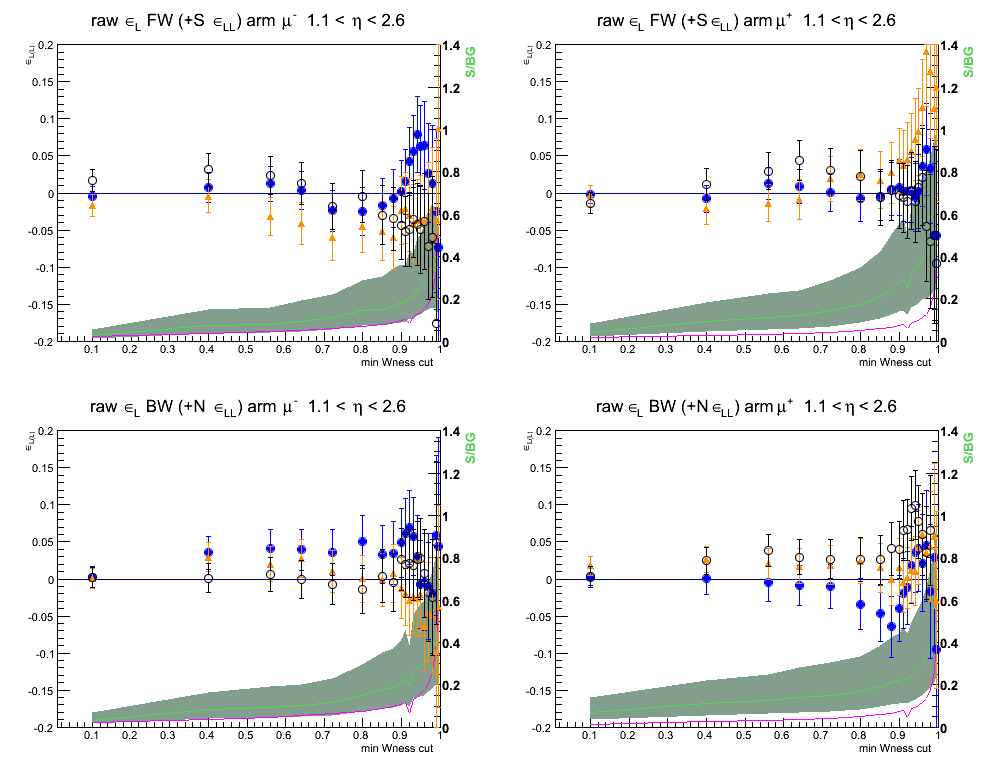
\includegraphics[width=\textwidth]{{./figures/asyvsfcut13_wness_eta3_16_60_dw2}.png}
\caption{
Raw asymmetries $\epsilon_{L}$ for the Blue (blue symbols) and Yellow (orange
symbols) beams and $\epsilon_{LL}$ (black symbols) for both arms and charges as
a function of the pre-selection range. The combination of all rapidities in one
bin after selecting the {\bf sideband} $dw_{23}$ region is displayed. In addition the
extracted signal to background ratios are displayed using the right-hand axis
values. The green line displays the data-based extraction method while the
magenta line represents the MC signal based extraction.\label{fig:dwcuts}
}
\end{center}
\end{figure}

\subsection{Asymmetries and Signal to BG ratio as a function of rate, time and transverse momentum range}
Another important test is whether the asymmetries show any kind of rate or run
dependence effect. For this purpose the data was split up into three rapidity
ranges with about equal luminosity: The multi-collision parameters were chosen
as 0, 0.69, 0.83, 2. Naively a rate dependent effect would result in a certain
ordering of the asymmetries with either increasing or decreasing asymmetries as
the rates increase. All the asymmetries as a function of minimum $W_{ness}$ cut are displayed in Fig.~\ref{fig:rateranges}. Out of the 12 different asymmetries ( arm x charge x singe,double spin asymmetry) a few display such a behavior while the majority appears to be randomly distributed between the different rates. 
\begin{figure}[ht] % %does not exists!
\begin{center}
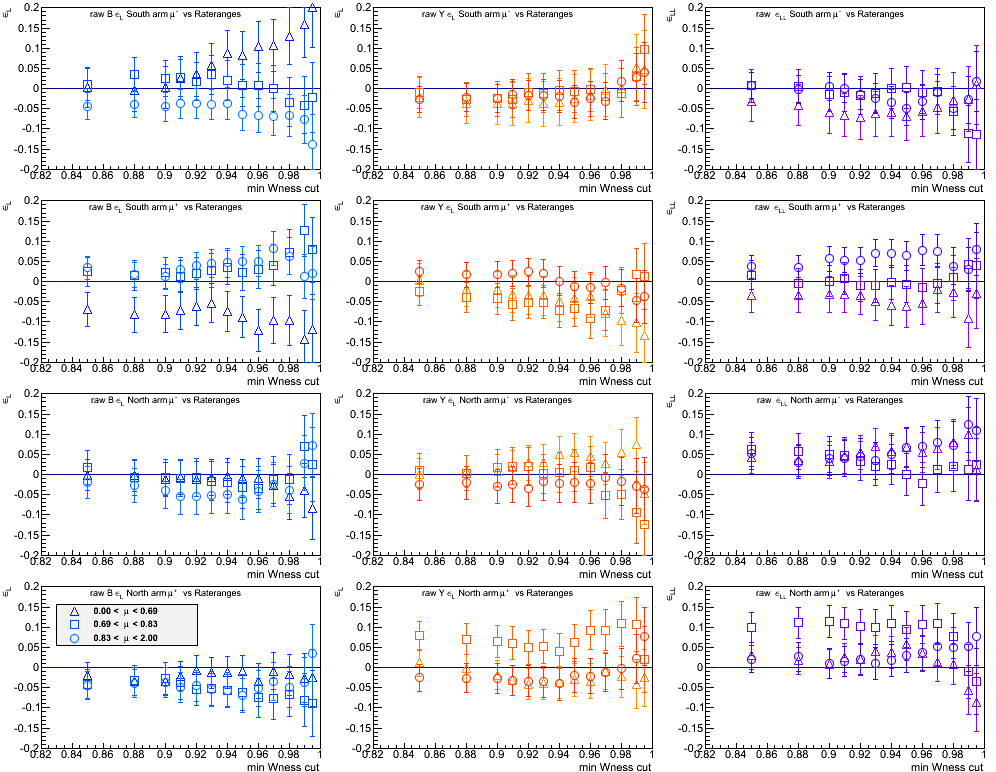
\includegraphics[width=\textwidth]{{./figures/asyvsfcut13_wness_16_60_dw6}.png}
\caption{Raw asymmetries as a function of minimal $W_{ness}$ cut when splitting the data sample into three nearly equal luminosity bins of increasing BBC rate in the order of open triangles, open squares and open circles. Each plot displays one asymmetry for each arm and charge. The central $dw_{23}$ region has been selected.  In addition the extracted signal to background ratios are displayed using the right-hand axis values. The green line displays the data-based extraction method while the magenta line represents the MC signal based extraction.\label{fig:rateranges}}
\end{center}
\end{figure}

A t-test between low and high to intermediate rates was performed and the distribution is given in Fig.~\ref{fig:raterangest}. The amount of larger differences is on the order expected for statistical fluctuations around an average value and therefore one can conclude, that no obvious rate dependent effect is visible.   
\begin{figure}[ht]
\begin{center}
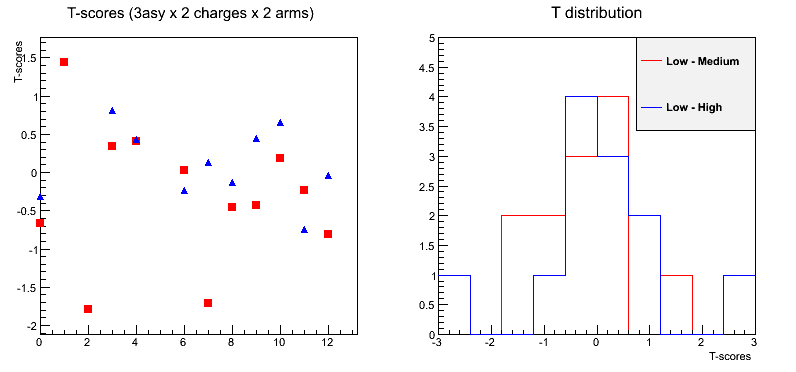
\includegraphics[width=\textwidth]{{./figures/tscores13_wness_16_60_dw6}.png}
\caption{Student T scores and distribution when comparing the lot to medium and the low to high rate subset.\label{fig:raterangest}}
\end{center}
\end{figure}

Similarly, the run dependence was studied in three range bins from 0, 392276, 395770, 399000. While some correlation with the rates is likely, it should be mostly washed out as the collision rates decrease within fills. With the run dependence it would be possible to see, if time dependent detector or accelerator related effects bias the results in some way. 
The resulting asymmetries can be seen in Fig.~\ref{fig:runranges} and the
corresponding t-test between low, high and mid run ranges is given in
Fig.~\ref{fig:runrangest}. Again, while some asymmetries show a range dependence
the overall distribution of differences as consistent with fluctuations only.  


\begin{figure}[ht] 
\begin{center}
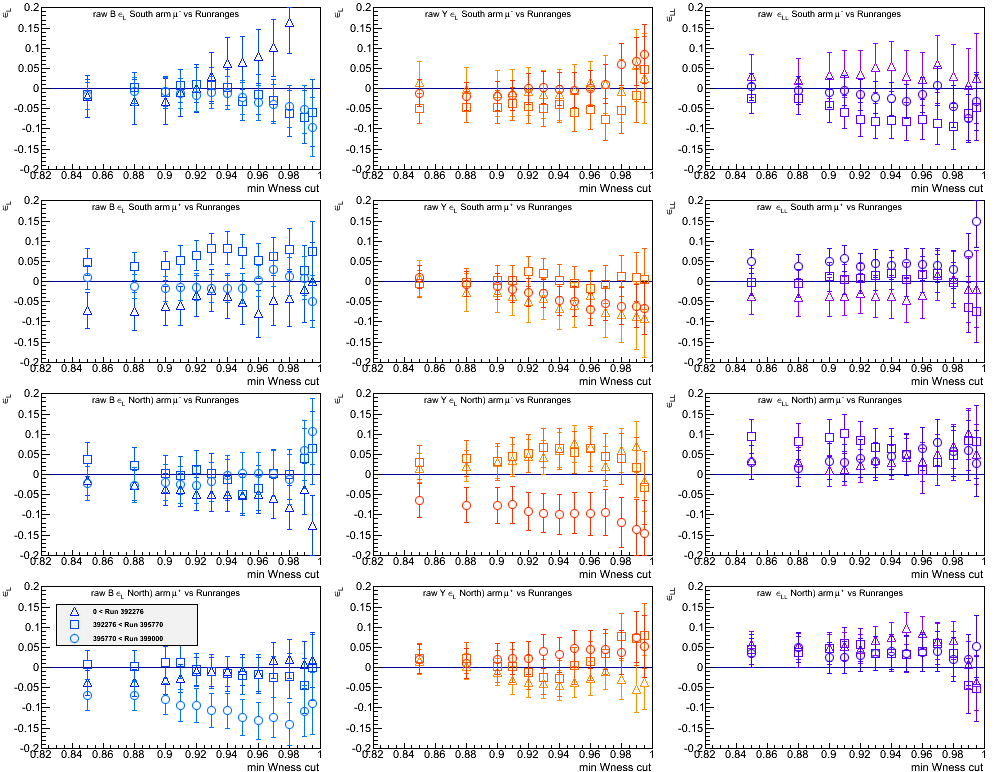
\includegraphics[width=\textwidth]{{./figures/asyvsfcut13_wness_16_60_dw3}.png}
\caption{Raw asymmetries as a function of minimal $W_{ness}$ cut when splitting the data sample into three nearly equal luminosity bins of increasing run number in the order of open triangles, open squares and open circles. Each plot displays one asymmetry for each arm and charge. The central $dw_{23}$ region has been selected.  In addition the extracted signal to background ratios are displayed using the right-hand axis values. The green line displays the data-based extraction method while the magenta line represents the MC signal based extraction.\label{fig:runranges}}
\end{center}
\end{figure}

\begin{figure}[ht]
\begin{center}
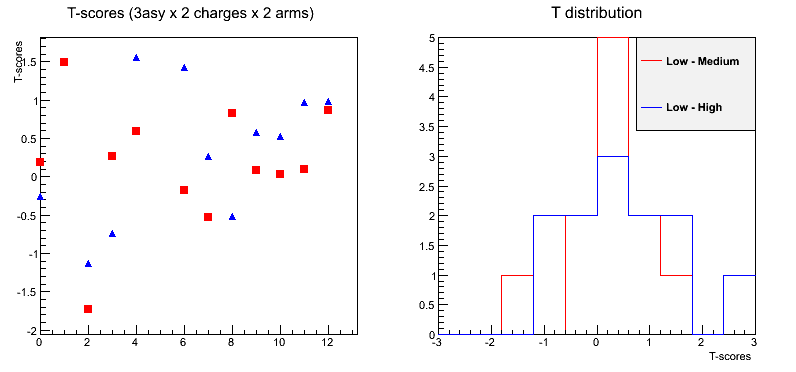
\includegraphics[width=\textwidth]{{./figures/tscores13_wness_16_60_dw3}.png}
\caption{Student T scores and distribution when comparing the lot to medium and the low to high run number subset}\label{fig:runrangest}
\end{center}
\end{figure}


Another test is the dependence on the minimum transverse momentum cut or the transverse momentum range selected. As mentioned earlier in this analysis note the W and Z decay muons dominate at larger transverse momenta while at lower transverse momenta even more dilution from other muon processes and fake hadrons contribute. As a consequence any asymmetry should be largely diluted and start to appear as the minimum transverse momentum cut is increased. 
Such a behavior can be seen in Fig.~\ref{fig:minptasymmetries} where essentially all asymmetries are consistent with zero at low transverse momenta and then increase in some of the cases. What appears different than expectation is the signal to background ratio obtained from the fits. The signal to background ratios from the fits seem to be not increasing while the MC based signal to background ratios show the expected behavior. 
\begin{figure}[ht] 
\begin{center}
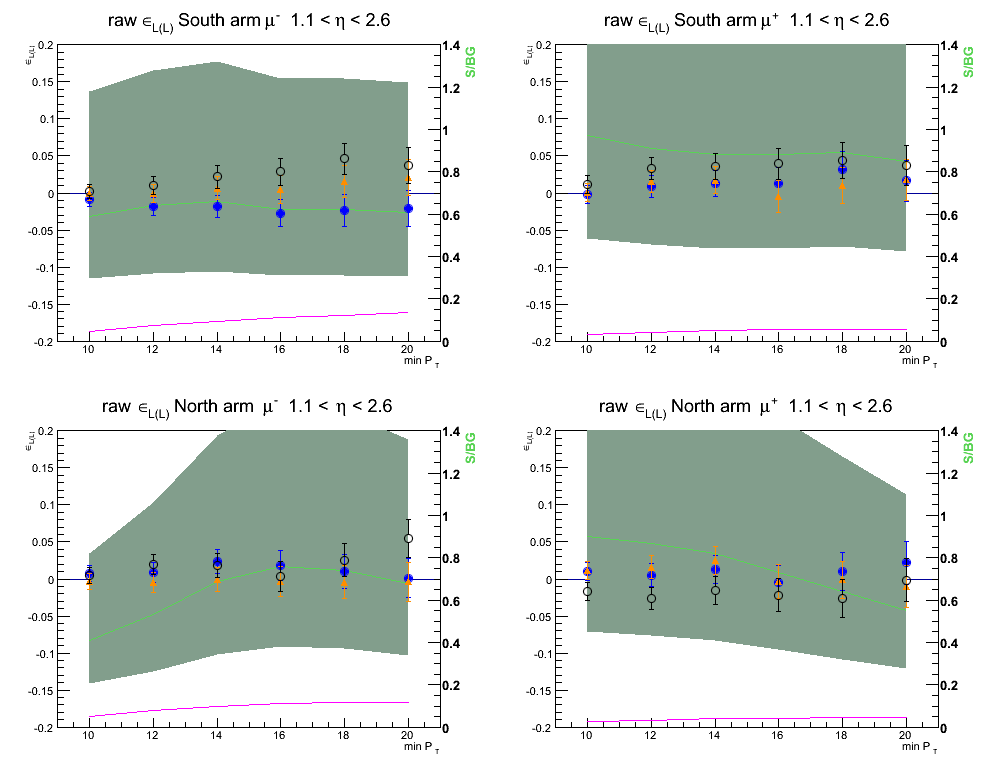
\includegraphics[width=\textwidth]{{./figures/asyvspt13_wness_eta3_0.920_dw0}.png}
\caption{Raw asymmetries $\epsilon_{L}$ for the Blue (blue symbols) and Yellow (orange symbols) beams and $\epsilon_{LL}$ (black symbols) for both arms and charges as a function of the minimal transverse momentum cut are displayed. In addition the extracted signal to background ratios are displayed using the right-hand axis values. The green line displays the data-based extraction method while the magenta line represents the MC signal based extraction.\label{fig:minptasymmetries}}
\end{center}
\end{figure}

The asymmetries in ranges of transverse momenta are shown in Fig.~
\ref{fig:rangeptasymmetries}. After small initial asymmetries they are mostly
consistent at intermediate transverse momentum ranges and only seem to change
again at transverse momenta of around 18. The signal-to-background distribution
is again unexpected as obtained from the fits while it is more consistent with
expectations in the MC based extraction.  
\begin{figure}[ht]  %does not exists!
\begin{center}
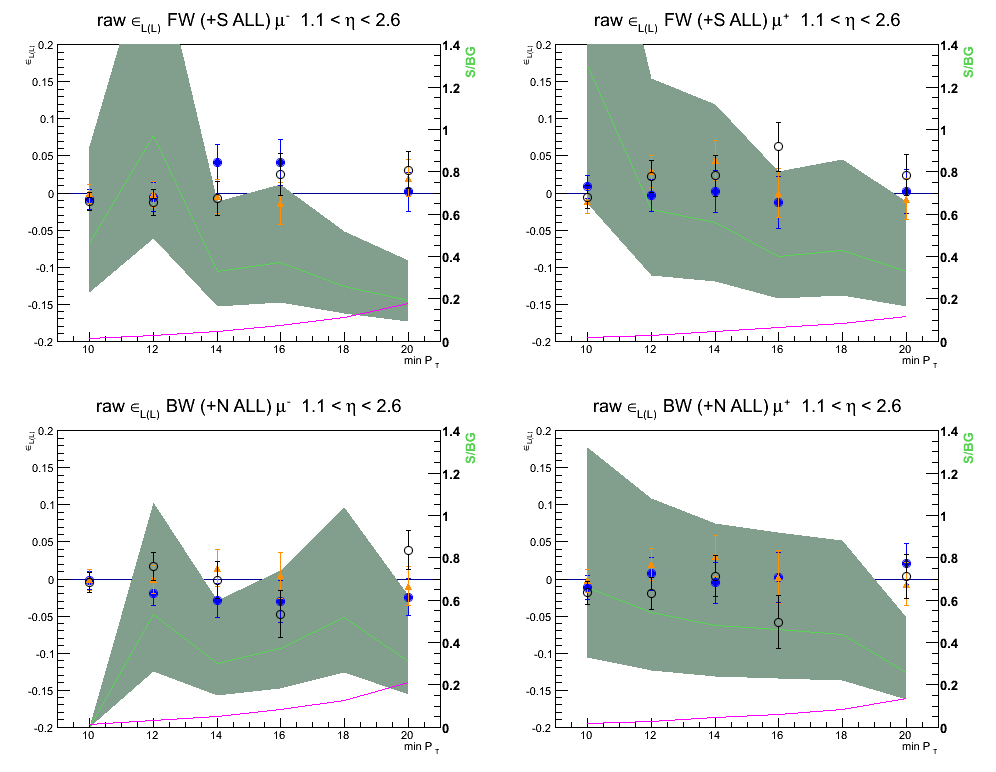
\includegraphics[width=\textwidth]{{./figures/asyvspt13ptslices_wness_eta3_0.920_dw0}.png}
\caption{Raw asymmetries $\epsilon_{L}$ for the Blue (blue symbols) and Yellow
(orange symbols) beams and $\epsilon_{LL}$ (black symbols) for both arms and
charges as a function of transverse momentum are displayed. The combination of
all rapidities in one bin after selecting the central $dw_{23}$ region is
displayed. In addition the extracted signal to background ratios are displayed
using the right-hand axis values. The green line displays the data-based
extraction method while the magenta line represents the MC signal based
extraction.\label{fig:rangeptasymmetries}}
\end{center}
\end{figure}


 \subsection{Addition of artificial MC-based signal and asymmetries}
Another type of test uses the generated signal MC and includes a fraction of it
into the data set before calculating asymmetries and signal to background
ratios. In order to do so, crossings are assigned randomly to the MC such, that a
certain set of asymmetries can be generated. As an initial test only constant
asymmetries were generated. Not any asymmetries can be physically created as the
yields in the 4 helicity combinations need to non-negative. The double spin
asymmetries need to be within a certain range of the other two.  
The initial asymmetries created were 40\% and 10\% for the negative generated
muons and -20\% and -30\% for the positive generated muons while no double spin
asymmetries were generated.

\begin{figure}[ht]  %does not exists!
\begin{center}
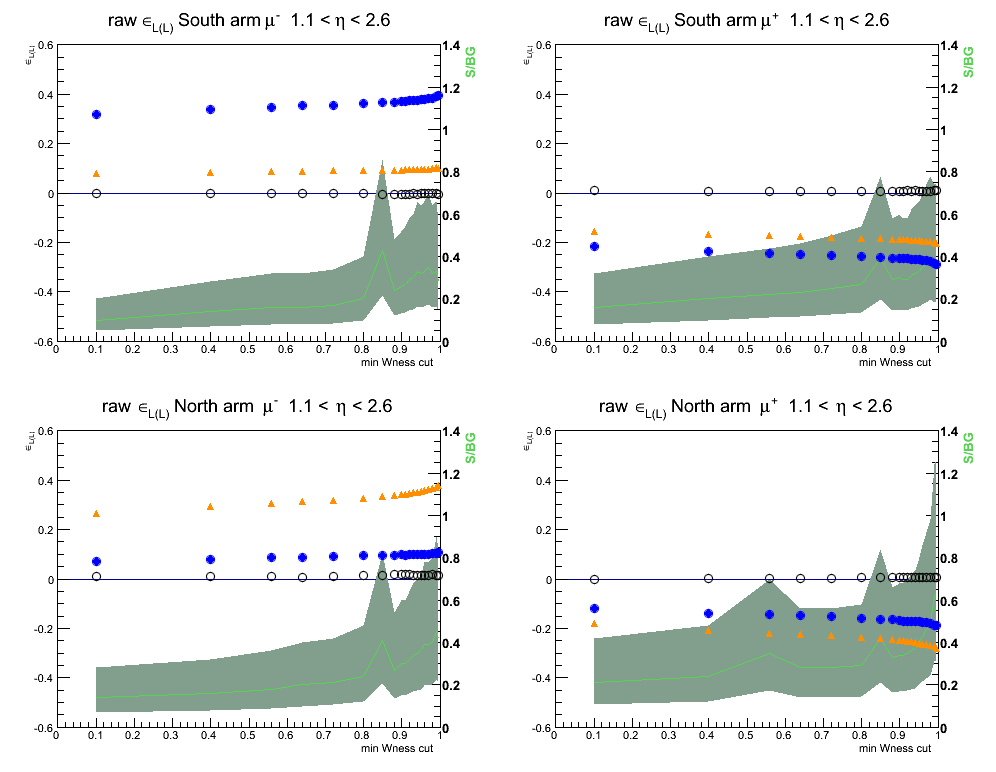
\includegraphics[width=\textwidth]{{./figures/asyvsfcut13_wness_eta3_16_dw1000}.png}
\caption{Raw asymmetries $\epsilon_{L}$ for the Blue (blue symbols) and Yellow (orange symbols) beams and $\epsilon_{LL}$ (black symbols) for both arms and charges as a function of the minimum $W_{ness}$ cut are displayed with a fixed signal MC addition of 20 fb$^{-1}$. The combination of all rapidities in one bin after selecting the central $dw_{23}$ region is displayed. In addition the extracted signal to background ratios are displayed using the right-hand axis values. The green line displays the data-based extraction method while the magenta line represents the MC signal based extraction. \label{fig:mcadd1}}
\end{center}
\end{figure}

The resulting asymmetries and signal-to-background ratios are displayed in Fig.~\ref{fig:mcadd1} for an MC admixture of 20 fb$^{-1}$ as a function of the minimum $W_{ness}$ cut. One can see, that with increasing minimum $W_{ness}$ the resulting asymmetries begin to increase as expected while the generally fall short of the generated asymmetries. In Fig.~\ref{fig:mcadd3} the asymmetries and signal-to-background ratios are displayed as a function of the MC admixture. Also the background corrected asymmetries are displayed which should return the generated asymmetries with the exception of the actual signal based asymmetries in the actual data.   
As one can see, the asymmetries are not properly recovered especially at low admixtures. While part of it could be coming from the Physics asymmetries its contribution should be small. Again, using the MC based signal to background ratios seem to better recover the generated asymmetries.   

\begin{figure}[ht] 
\begin{center}
%\includegraphics[width=\textwidth]{{./figures/asyvsmcaddition_wness_eta3_0.920_dw1000_corr}.png}
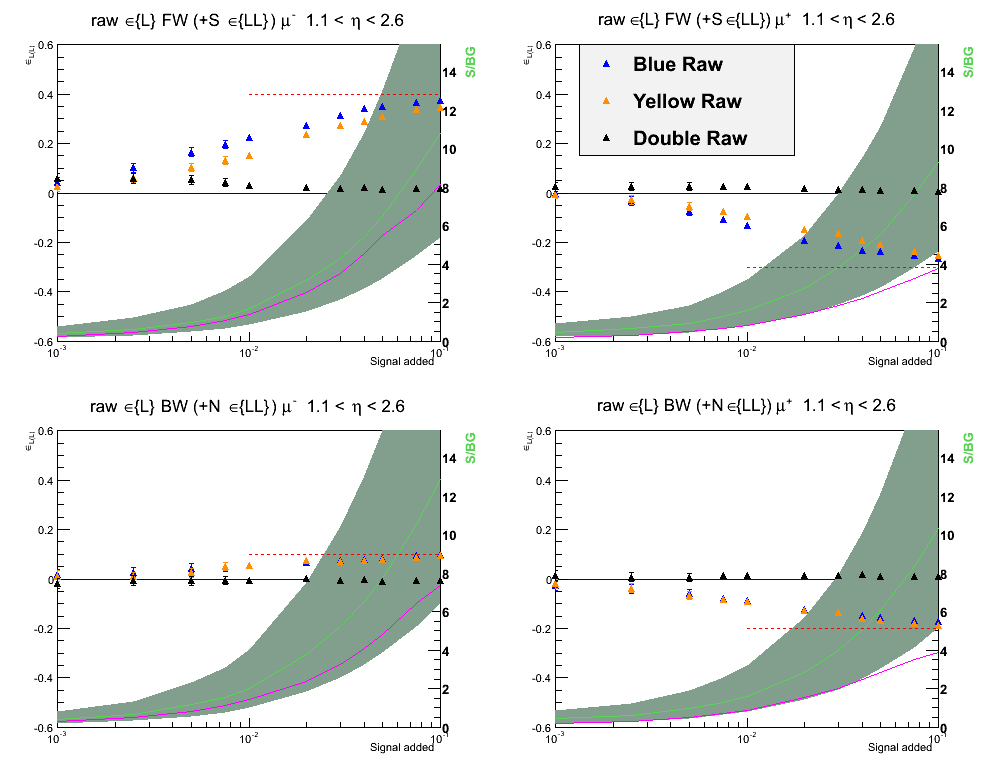
\includegraphics[width=\textwidth]{{./figures/asyvsmcaddition_wness_eta3_0.920_dw1000}.png}
\caption{Raw asymmetries $\epsilon_{L}$ for the Blue (blue symbols) and Yellow (orange symbols) beams and $\epsilon_{LL}$ (black symbols) for both arms and charges as a function of the total Signal MC added are displayed. The combination of all rapidities in one bin after selecting the central $dw_{23}$ region is displayed. In addition the extracted signal to background ratios are displayed using the right-hand axis values. The green line displays the data-based extraction method while the magenta line represents the MC signal based extraction. The background corrected asymmetries using either the fit based S/BG values (downward open triangles) or old extraction (upward open triangles) are also displayed.\label{fig:mcadd3}}
\end{center}
\end{figure}



 
\subsection{Checking the relative luminosities between patterns}
In the previous evaluation of the asymmetries we were implicitly assuming that we took the same luminosity for every spin pattern.
To make sure this is the case, we explicitly counted the scalers from the spin Data Base from the entry ScalerBbcNoCut for each spin pattern and we found the following:
%\begin{table}
\begin{center}
\begin{tabular}{|c|c|}
Spin Pattern (Blue, Yellow) & \\
\hline 
+1, +1 & 5.29+11\\
-1, +1 & 5.28e+11\\
+1, -1 & 5.29e+11\\
-1, -1 & 5.29e+11.\\
\hline 
%\caption{Scalers count for every spin pattern.}
\end{tabular}
\end{center}
%\end{table}
As can be seen in the previous table, there is only a 0.2\% difference between the luminosity of the spin patterns,
so the previous assumption that there are no differences in luminosities between spin patterns is safe. As a double check,
we rescaled the yield for each spin pattern according to the scalers just reported, and as expected no significant differences
were observed in the combined asymmetries, as shown in figure~\ref{fig:asyscaled}.

\begin{figure}[ht]
\begin{center}
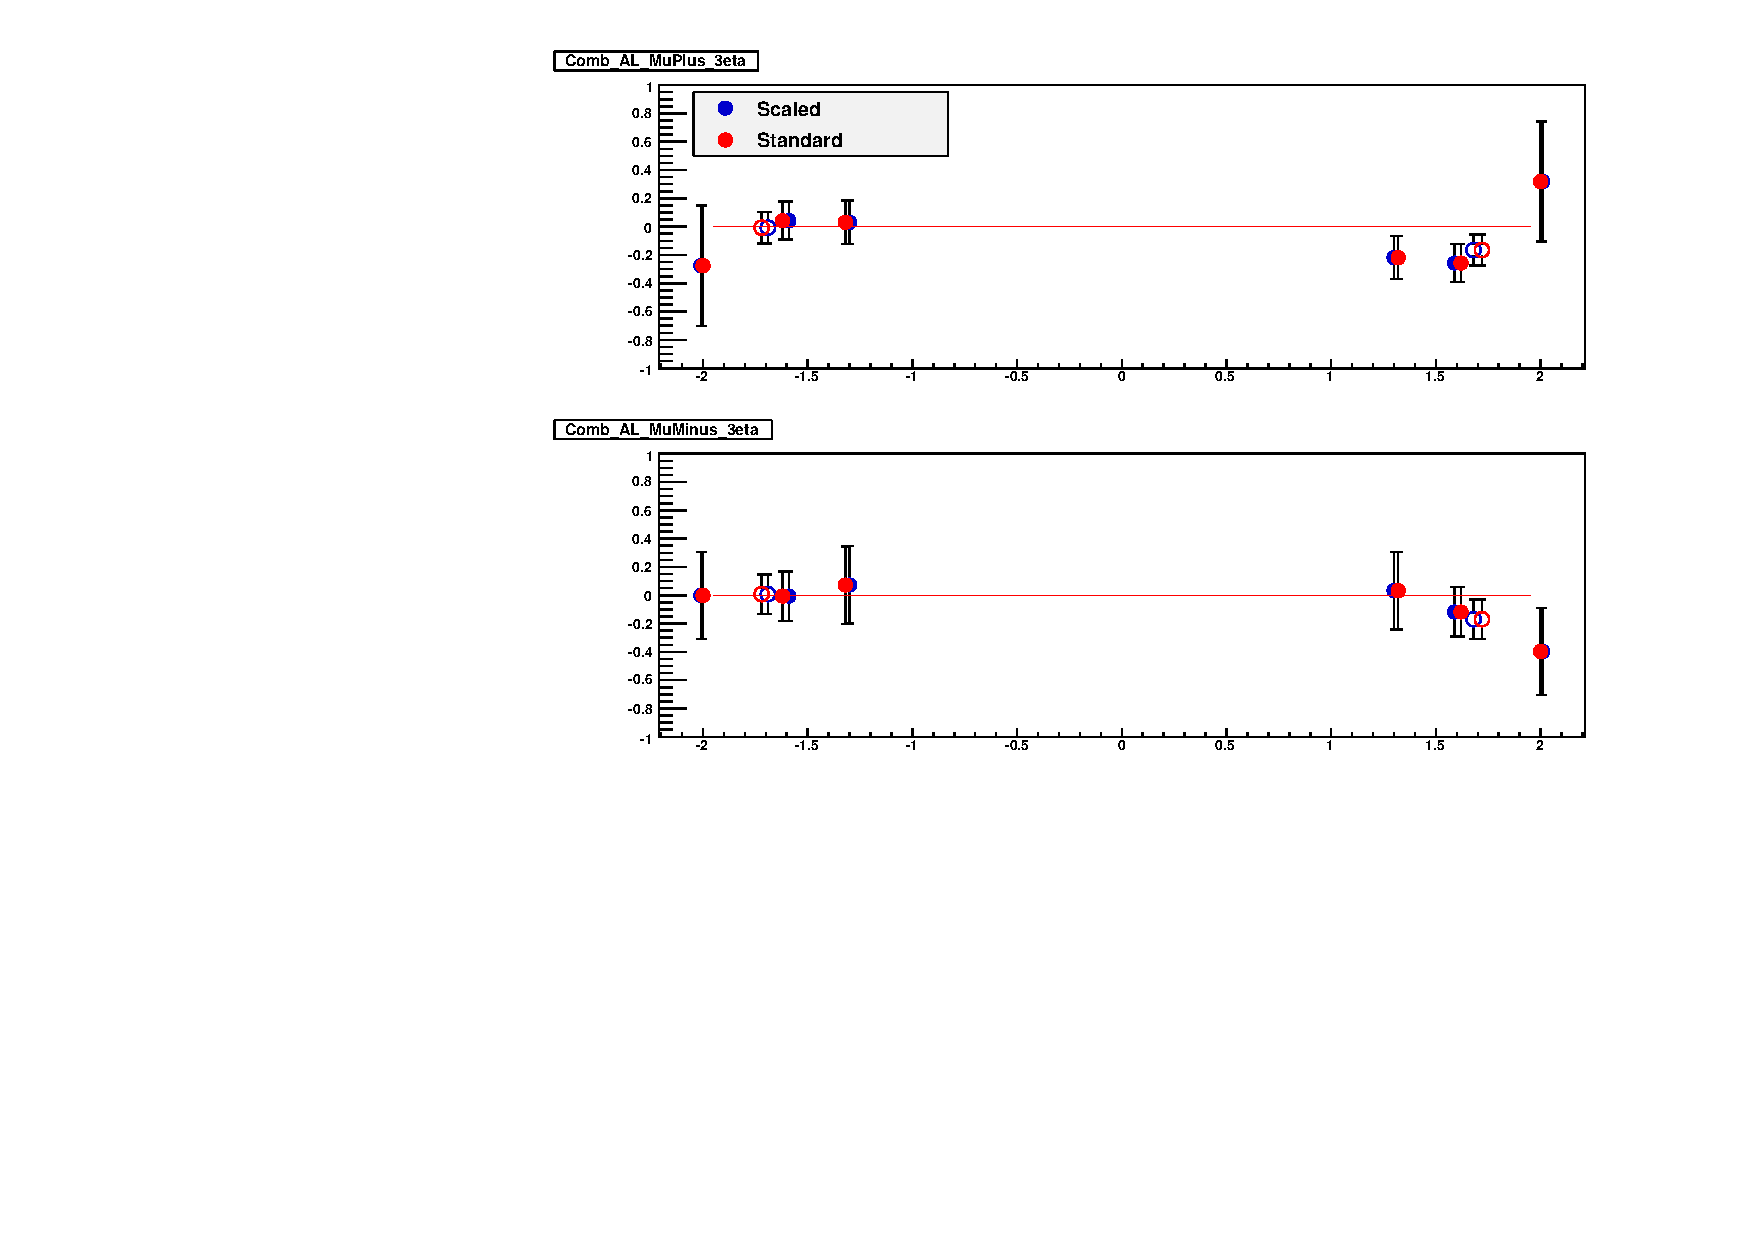
\includegraphics[width=\textwidth]{{./figures/combined_asy_scaled}.pdf}
\caption{Comparison between the combined asymmetries with (in blue) and without (in red) the yield rescaling 
by the relative luminosity of each spin pattern.}
\label{fig:asyscaled}
\end{center}
\end{figure}
